\documentclass[11pt]{article}
\usepackage[margin=1in]{geometry}
\usepackage{listings}
\usepackage{xcolor}
\usepackage{graphicx}
\usepackage{enumitem}
\usepackage{amsmath}

\lstset{
  basicstyle=\ttfamily\footnotesize,
  commentstyle=\color{gray},
  language=C++,
  breaklines=true,
  showstringspaces=false
}

\setlength{\parindent}{0pt}
\setlength{\parskip}{8pt}

\begin{document}

Karishma Premnath \\
EECE 7205, Stacks and Queues, In-Class Work

\hrulefill

{\large \textbf{Problem 1. Expression Evaluation Using Stacks}}

\textbf{(a) Functions}

\begin{itemize}[leftmargin=*, itemsep=2pt, topsep=2pt]
\item \texttt{isNumber(s)} \quad a token is a number if it is all digits, or a minus sign
      followed by digits. This is how \texttt{-7} is read as a value and not as subtraction.
\item \texttt{toInt(s)} \quad converts a number token to an \texttt{int}, handling the
      leading minus sign.
\item \texttt{precedence(c)} \quad \texttt{\^{}} is 3, \texttt{*} and \texttt{/} are 2,
      \texttt{+} and \texttt{-} are 1.
\item \texttt{floorDiv(a, b)} \quad rounds down toward negative infinity by subtracting one
      when the signs differ and the division is not exact.
\item \texttt{applyOp(a, b, c)} \quad does one operation on two integers, with \texttt{a} as
      the left operand. Division calls \texttt{floorDiv}.
\item \texttt{evaluate(tok)} \quad pushes values on the values stack, and before pushing an
      operator it applies every waiting operator that must go first.
\item \texttt{ValueStack} and \texttt{OpStack} \quad the two stacks, one holding \texttt{int}
      values and one holding \texttt{char} operators.
\end{itemize}

\textbf{(b) Evaluate \texttt{8 + 3 * 2 \^{} 2 - 20 / 4}}

\begin{tabular}{llll}
Step & Operator & Calculation & Expression left \\[2pt]
\hline
    &            &                 & \texttt{8 + 3 * 2 \^{} 2 - 20 / 4} \\
1 & \texttt{\^{}} & \texttt{2 \^{} 2 = 4}   & \texttt{8 + 3 * 4 - 20 / 4} \\
2 & \texttt{*}    & \texttt{3 * 4 = 12}  & \texttt{8 + 12 - 20 / 4} \\
3 & \texttt{/}    & \texttt{20 / 4 = 5}       & \texttt{8 + 12 - 5} \\
4 & \texttt{+}    & \texttt{8 + 12 = 20}      & \texttt{20 - 5} \\
5 & \texttt{-}    & \texttt{20 - 5 = 15}      & \texttt{15} \\
\end{tabular}

Step 1 goes first because \texttt{\^{}} has the highest precedence. Steps 2 and 3 come next
and are taken left to right, then steps 4 and 5 the same way.

\textbf{Answer: 15}

\textbf{(c) Trace}

The two stacks after each token is processed:

\begin{tabular}{llll}
Token & Action & Values (bottom to top) & Operators \\[2pt]
\hline
\texttt{8}  & push 8 & 8 & \\
\texttt{+}  & push \texttt{+} & 8 & \texttt{+} \\
\texttt{3}  & push 3 & 8 3 & \texttt{+} \\
\texttt{*}  & push \texttt{*} & 8 3 & \texttt{+ *} \\
\texttt{2}  & push 2 & 8 3 2 & \texttt{+ *} \\
\texttt{\^{}}  & push \texttt{\^{}} & 8 3 2 & \texttt{+ * \^{}} \\
\texttt{2}  & push 2 & 8 3 2 2 & \texttt{+ * \^{}} \\
\texttt{-}  & apply \texttt{\^{}}, \texttt{*}, \texttt{+}, then push \texttt{-} & 20 & \texttt{-} \\
\texttt{20} & push 20 & 20 20 & \texttt{-} \\
\texttt{/}  & push \texttt{/} & 20 20 & \texttt{- /} \\
\texttt{4}  & push 4 & 20 20 4 & \texttt{- /} \\
\end{tabular}

At token \texttt{-}, three operators are applied because \texttt{-} has lower precedence than
all three operators on the stack:

\begin{tabular}{lll}
Apply & Calculation & Values after \\[2pt]
\hline
\texttt{\^{}} & \texttt{2 \^{} 2 = 4} & 8 3 4 \\
\texttt{*}    & \texttt{3 * 4 = 12} & 8 12 \\
\texttt{+}    & \texttt{8 + 12 = 20} & 20 \\
\end{tabular}

Remaining calculations once the tokens are finished:

\begin{tabular}{lll}
Apply & Calculation & Values after \\[2pt]
\hline
\texttt{/} & \texttt{20 / 4 = 5} & 20 5 \\
\texttt{-} & \texttt{20 - 5 = 15} & 15 \\
\end{tabular}

\textbf{Result: 15}

\textbf{(d) Tests}

\begin{tabular}{lll}
Expression & Answer & Common wrong answer \\[2pt]
\hline
\texttt{2 \^{} 3 \^{} 2} & 512 & 64 \\
\texttt{-7 / 2} & $-4$ & $-3$ \\
\end{tabular}

\texttt{2 \^{} 3 \^{} 2} gives \textbf{512}. When the second \texttt{\^{}} arrives, the first one has
equal precedence, and \texttt{\^{}} is right associative, so it is left waiting instead of being
applied. That makes \texttt{3 \^{} 2 = 9} run first, then \texttt{2 \^{} 9 = 512}. Treating \texttt{\^{}} as
left associative would give \texttt{(2 \^{} 3) \^{} 2 = 64}.

\texttt{-7 / 2} gives \textbf{-4}. The exact value is $-3.5$. C++ integer division cuts the fraction
off toward zero and gives $-3$, but the question asks for rounding down toward negative
infinity, which is $-4$. \texttt{floorDiv} subtracts one because the signs differ and the
division is not exact. A clean division such as $-20 / 4$ is untouched and stays $-5$.

\newpage
\textbf{Code}

\lstinputlisting{expression_eval_short.cpp}

\begin{minipage}{\linewidth}
\textbf{Output}

\vspace{4pt}
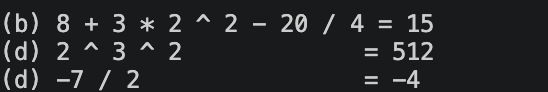
\includegraphics[width=\linewidth]{q1_output.png}
\end{minipage}

\newpage

{\large \textbf{Problem 2. Logic Gate Analysis and Implementation}}

\textbf{(a) Circuit and intermediate signals}

Four levels, eight gates:

\begin{tabular}{llll}
Level & Gate & Inputs & Output label \\[2pt]
\hline
1 & NOT & $C$ & $N_1$ \\
1 & NOT & $D$ & $N_2$ \\
2 & OR & $B$, $N_1$ & $P$ \\
2 & OR & $C$, $N_2$ & $R$ \\
3 & AND & $A$, $P$ & $Q$ \\
3 & AND & $B$, $R$ & $S$ \\
3 & AND & $A$, $D$ & $T$ \\
4 & OR (3 input) & $Q$, $S$, $T$ & $Z$ \\
\end{tabular}

Each input is used twice: $A$ feeds $Q$ and $T$, $B$ feeds $P$ and $S$, $C$ feeds $N_1$
and $R$, $D$ feeds $N_2$ and $T$.

\begin{center}
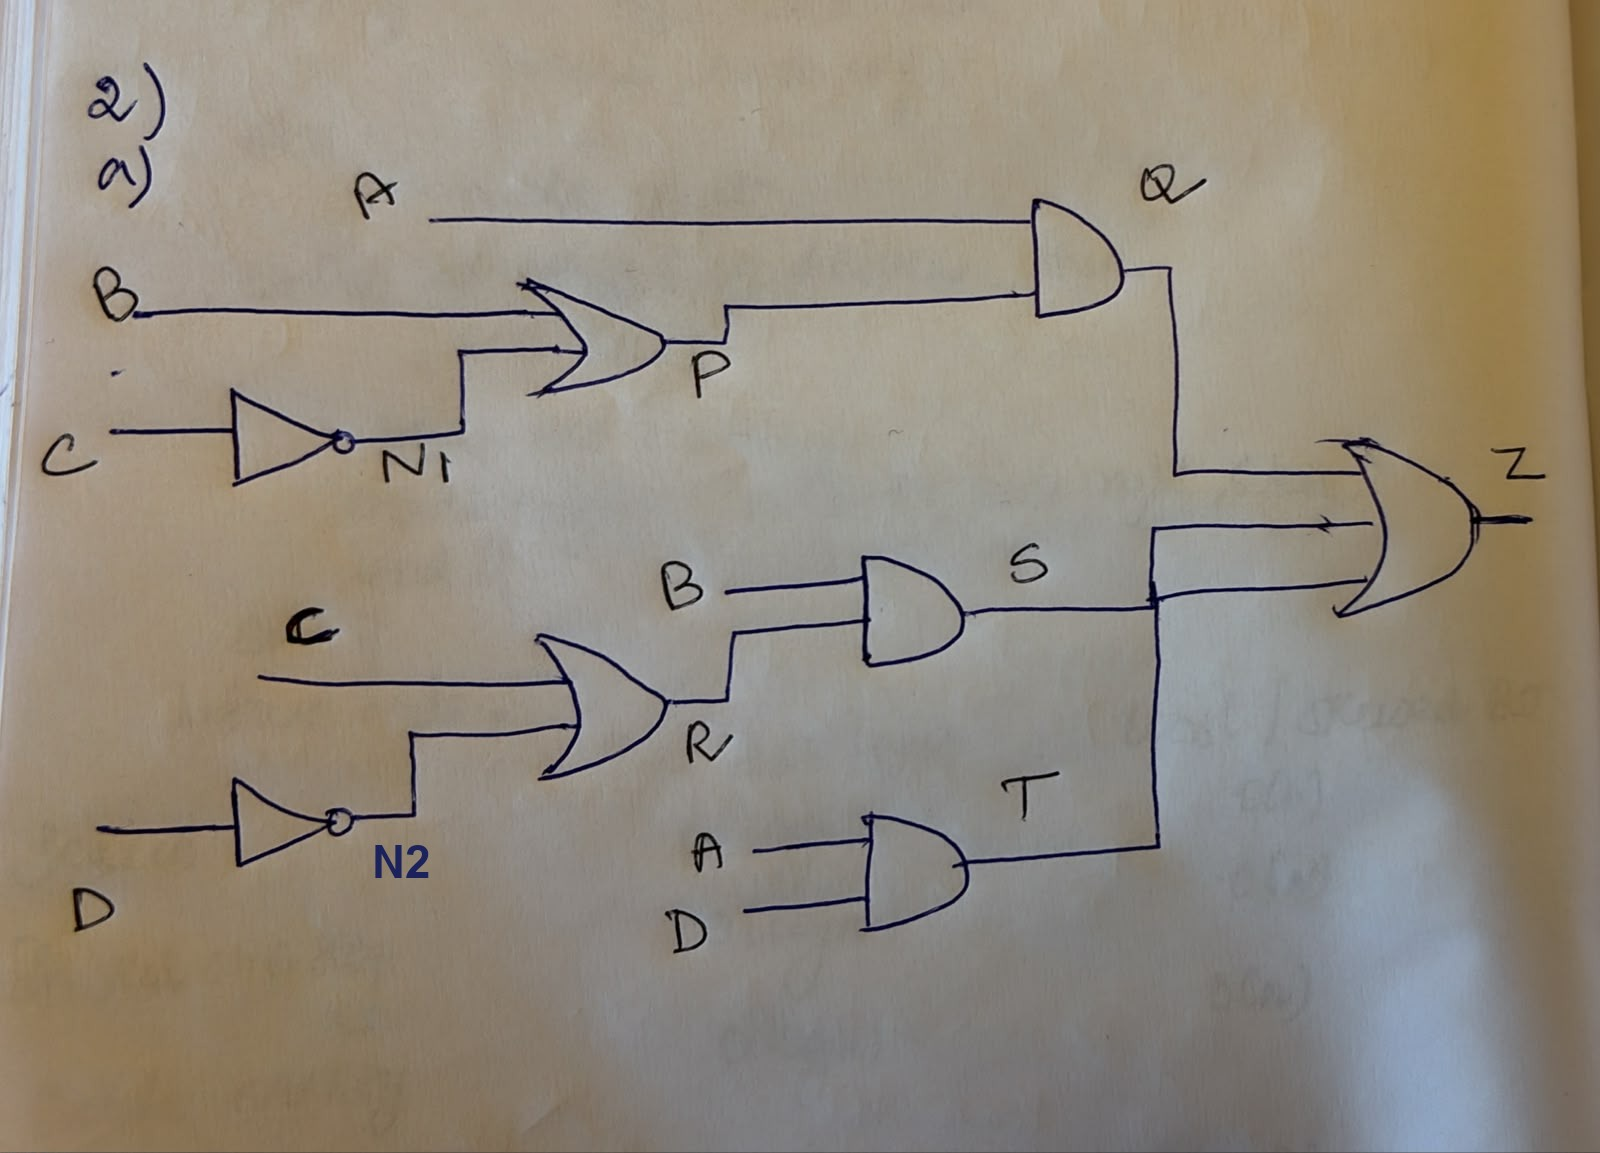
\includegraphics[width=0.92\linewidth]{q2a_hand_labeled.jpg}
\end{center}

\begin{center}
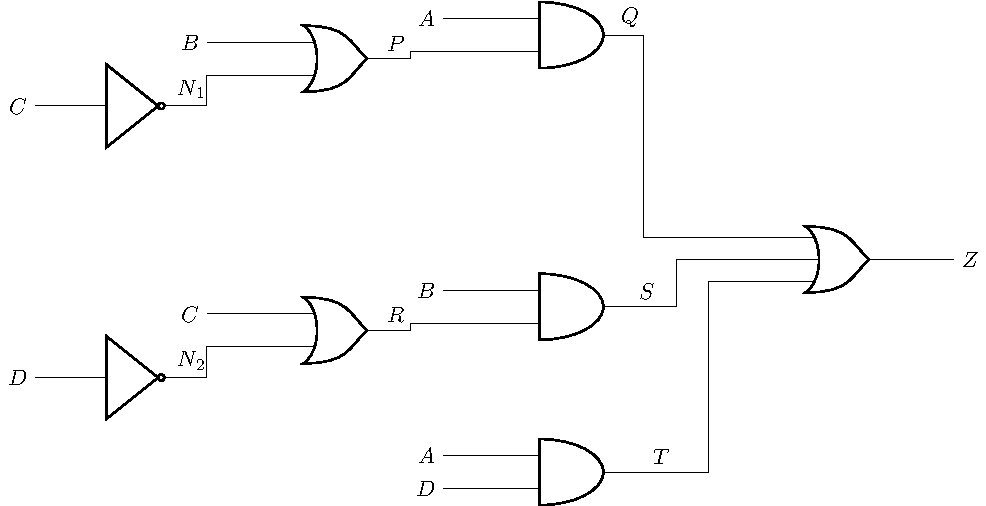
\includegraphics[width=\linewidth]{q2_circuit_ref.pdf}
\end{center}

\textbf{(b) Boolean expression}

Working through the gate list in order:

\begin{align*}
N_1 &= C' \\
N_2 &= D' \\
P &= B + C' \\
Q &= A(B + C') \\
R &= C + D' \\
S &= B(C + D') \\
T &= AD \\
Z &= Q + S + T = A(B + C') + B(C + D') + AD
\end{align*}

Multiplied out:
\[ Z = AB + AC' + BC + BD' + AD \]

\textbf{(c) Truth table}

\begin{tabular}{cccc|ccccccc|c}
$A$ & $B$ & $C$ & $D$ & $N_1$ & $N_2$ & $P$ & $Q$ & $R$ & $S$ & $T$ & $Z$ \\
\hline
0 & 0 & 0 & 0 & 1 & 1 & 1 & 0 & 1 & 0 & 0 & \textbf{0} \\
0 & 0 & 0 & 1 & 1 & 0 & 1 & 0 & 0 & 0 & 0 & \textbf{0} \\
0 & 0 & 1 & 0 & 0 & 1 & 0 & 0 & 1 & 0 & 0 & \textbf{0} \\
0 & 0 & 1 & 1 & 0 & 0 & 0 & 0 & 1 & 0 & 0 & \textbf{0} \\
0 & 1 & 0 & 0 & 1 & 1 & 1 & 0 & 1 & 1 & 0 & \textbf{1} \\
0 & 1 & 0 & 1 & 1 & 0 & 1 & 0 & 0 & 0 & 0 & \textbf{0} \\
0 & 1 & 1 & 0 & 0 & 1 & 1 & 0 & 1 & 1 & 0 & \textbf{1} \\
0 & 1 & 1 & 1 & 0 & 0 & 1 & 0 & 1 & 1 & 0 & \textbf{1} \\
1 & 0 & 0 & 0 & 1 & 1 & 1 & 1 & 1 & 0 & 0 & \textbf{1} \\
1 & 0 & 0 & 1 & 1 & 0 & 1 & 1 & 0 & 0 & 1 & \textbf{1} \\
1 & 0 & 1 & 0 & 0 & 1 & 0 & 0 & 1 & 0 & 0 & \textbf{0} \\
1 & 0 & 1 & 1 & 0 & 0 & 0 & 0 & 1 & 0 & 1 & \textbf{1} \\
1 & 1 & 0 & 0 & 1 & 1 & 1 & 1 & 1 & 1 & 0 & \textbf{1} \\
1 & 1 & 0 & 1 & 1 & 0 & 1 & 1 & 0 & 0 & 1 & \textbf{1} \\
1 & 1 & 1 & 0 & 0 & 1 & 1 & 1 & 1 & 1 & 0 & \textbf{1} \\
1 & 1 & 1 & 1 & 0 & 0 & 1 & 1 & 1 & 1 & 1 & \textbf{1} \\
\end{tabular}

$Z = 1$ for ten input combinations: $m_4$, $m_6$, $m_7$, $m_8$, $m_9$, $m_{11}$,
$m_{12}$, $m_{13}$, $m_{14}$, $m_{15}$.

\textbf{(d) Karnaugh map and minimum SOP}

Rows $AB$ and columns $CD$, both in Gray-code order, with the four groups looped:

\begin{center}
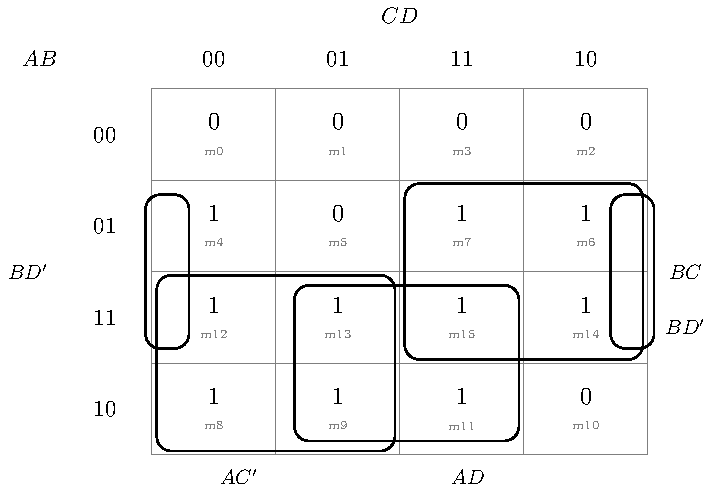
\includegraphics[width=0.95\linewidth]{q2_kmap.pdf}
\end{center}

Four groups of four cells:

\begin{tabular}{lll}
Group & Cells & Term \\[2pt]
\hline
$B=1$, $D=0$ & $m_4$, $m_6$, $m_{12}$, $m_{14}$ & $BD'$ \\
$B=1$, $C=1$ & $m_6$, $m_7$, $m_{14}$, $m_{15}$ & $BC$ \\
$A=1$, $D=1$ & $m_9$, $m_{11}$, $m_{13}$, $m_{15}$ & $AD$ \\
$A=1$, $C=0$ & $m_8$, $m_9$, $m_{12}$, $m_{13}$ & $AC'$ \\
\end{tabular}

\[ \boxed{Z = BD' + BC + AD + AC'} \]

The $BD'$ group wraps around the map. Its four cells are the two in the $CD=00$ column and
the two in the $CD=10$ column. Those columns are next to each other in Gray-code order, so
the group is legal even though it is drawn at the two edges.

$AB$ is also a prime implicant, covering $m_{12}$, $m_{13}$, $m_{14}$, $m_{15}$, but it is
redundant because all four of those cells are already covered by the groups above.
This four-term answer is the only minimum SOP.

\textbf{(e) NAND-only implementation}

Starting from $Z = BD' + BC + AD + AC'$. Each product term becomes a NAND gate. The two
partial sums are inverted, and a final NAND joins them. A NAND with both inputs tied
together acts as an inverter. Eleven two-input NAND gates:

\begin{tabular}{llll}
Gate & Inputs & Output & Meaning \\[2pt]
\hline
1  & $C$, $C$ & $C'$ & inverter \\
2  & $D$, $D$ & $D'$ & inverter \\
3  & $B$, $D'$ & $g_1$ & $(BD')'$ \\
4  & $B$, $C$ & $g_2$ & $(BC)'$ \\
5  & $A$, $D$ & $g_3$ & $(AD)'$ \\
6  & $A$, $C'$ & $g_4$ & $(AC')'$ \\
7  & $g_1$, $g_2$ & $X$ & $BD' + BC$ \\
8  & $g_3$, $g_4$ & $Y$ & $AD + AC'$ \\
9  & $X$, $X$ & $X'$ & inverter \\
10 & $Y$, $Y$ & $Y'$ & inverter \\
11 & $X'$, $Y'$ & $Z$ & $X + Y$ \\
\end{tabular}

\begin{center}
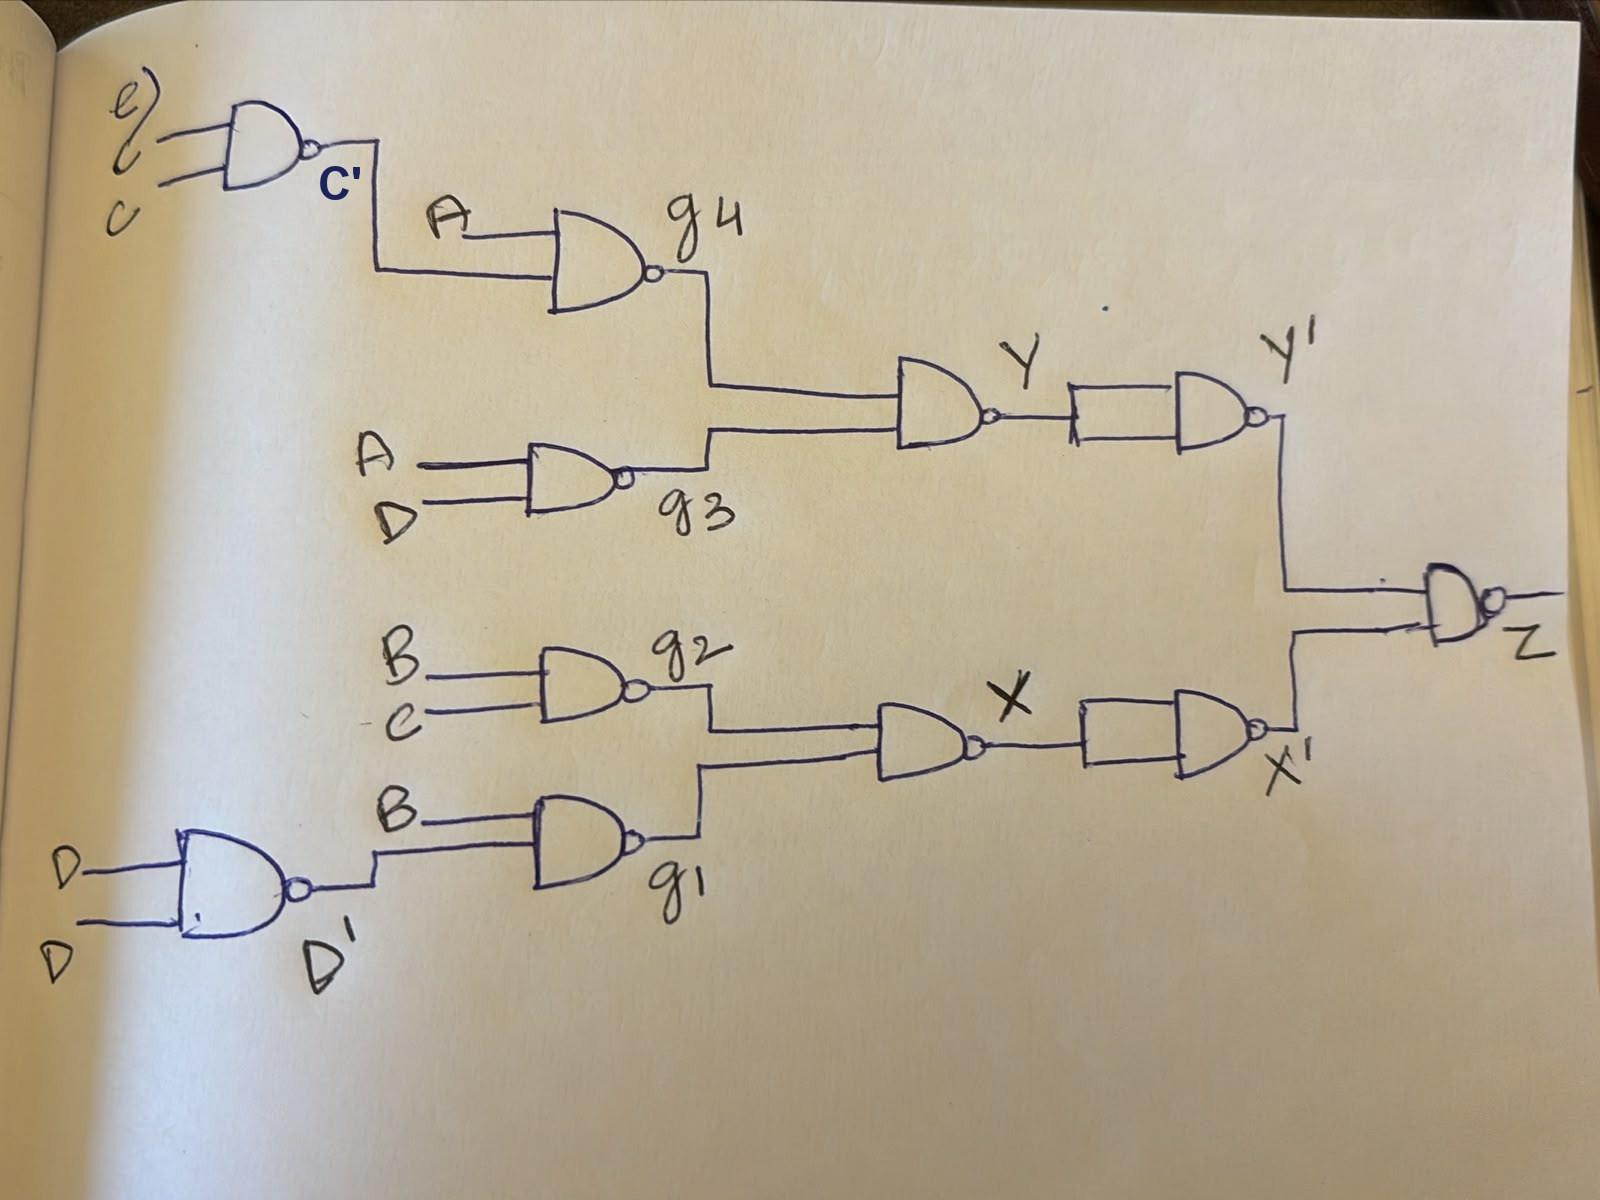
\includegraphics[width=0.92\linewidth]{q2e_hand_labeled.jpg}
\end{center}

\begin{center}
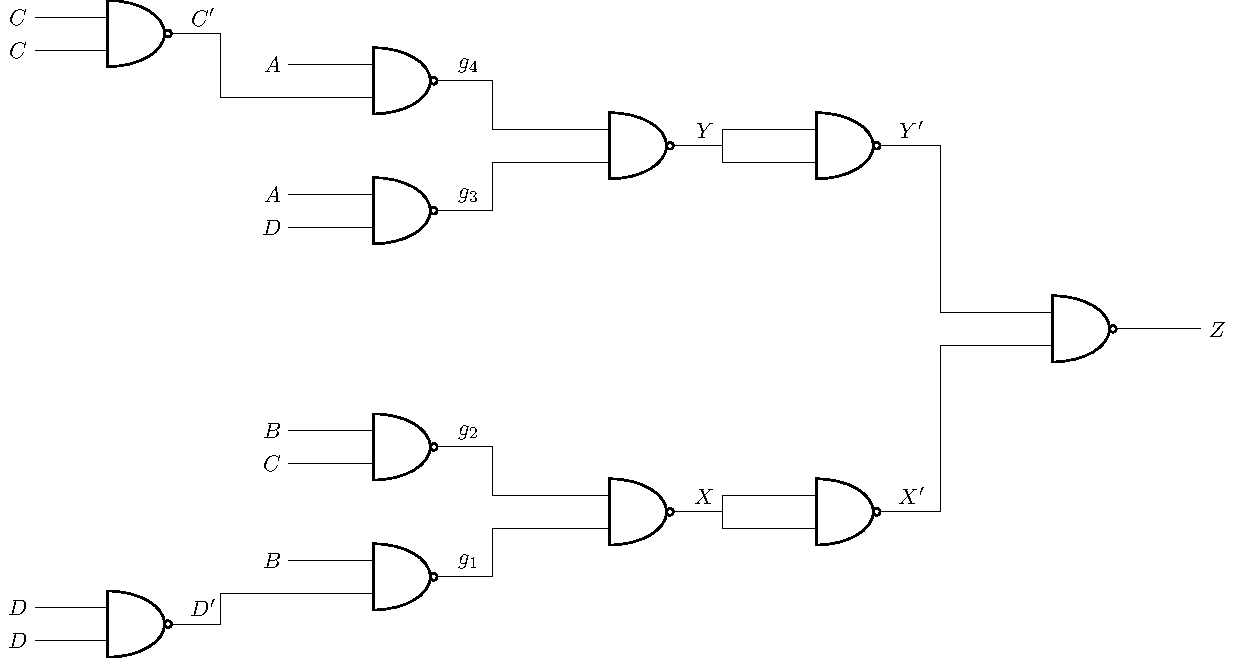
\includegraphics[width=\linewidth]{q2_nand_ref.pdf}
\end{center}

The program on the last page simulates these eleven NAND gates alongside the gate network,
in the \texttt{Z nand} column. The two agree on all sixteen rows.

\textbf{(f) Worst-case propagation delay}

Every NAND gate has a delay of 20 ns, so the delay of a path is 20 ns times the
number of gates on it.

\begin{tabular}{lll}
Path & Gates & Delay \\[2pt]
\hline
$C \rightarrow C' \rightarrow g_4 \rightarrow Y \rightarrow Y' \rightarrow Z$ & 5 & 100 ns \\
$D \rightarrow D' \rightarrow g_1 \rightarrow X \rightarrow X' \rightarrow Z$ & 5 & 100 ns \\
$A \rightarrow g_3 \rightarrow Y \rightarrow Y' \rightarrow Z$ & 4 & 80 ns \\
$B \rightarrow g_2 \rightarrow X \rightarrow X' \rightarrow Z$ & 4 & 80 ns \\
\end{tabular}

The longest input-to-output path is five gates, so the worst-case propagation delay is

\[ 5 \times 20\ \text{ns} = 100\ \text{ns} \]

reached from inputs $C$ and $D$, because those two have to pass through an inverter before
reaching a product gate. Inputs $A$ and $B$ are used uncomplemented and reach the output in
four gates.

\newpage
\textbf{Evaluating the expression with a stack}

The minimized expression is a sum of products, so it needs no parentheses and runs on the
same two-stack evaluator as Q1. The values stack holds 0 and 1, the operators stack holds
\texttt{\&} and \texttt{|}, and \texttt{\&} has higher precedence than \texttt{|}. A token
like \texttt{C'} is read as the complement of $C$.

\begin{lstlisting}[language=]
part (b):  A & B | A & C' | B & C | B & D' | A & D
part (d):  B & D' | B & C | A & D | A & C'
\end{lstlisting}

The program evaluates the part (b) expression and the part (d) minimized expression for all
sixteen input combinations, simulates the part (e) NAND circuit, and compares all three
against the original gate network.

Traced by hand for one input row, $A=1$, $B=0$, $C=1$, $D=1$, so $C'=0$ and $D'=0$:

\begin{tabular}{llll}
Token & Action & Values (bottom to top) & Operators \\[2pt]
\hline
\texttt{B}  & push 0 & 0 & \\
\texttt{\&} & push \texttt{\&} & 0 & \texttt{\&} \\
\texttt{D'} & push 0 & 0 0 & \texttt{\&} \\
\texttt{|}  & apply $0 \wedge 0 = 0$, push \texttt{|} & 0 & \texttt{|} \\
\texttt{B}  & push 0 & 0 0 & \texttt{|} \\
\texttt{\&} & push \texttt{\&} & 0 0 & \texttt{| \&} \\
\texttt{C}  & push 1 & 0 0 1 & \texttt{| \&} \\
\texttt{|}  & apply $0 \wedge 1 = 0$, then $0 \vee 0 = 0$, push \texttt{|} & 0 & \texttt{|} \\
\texttt{A}  & push 1 & 0 1 & \texttt{|} \\
\texttt{\&} & push \texttt{\&} & 0 1 & \texttt{| \&} \\
\texttt{D}  & push 1 & 0 1 1 & \texttt{| \&} \\
\texttt{|}  & apply $1 \wedge 1 = 1$, then $0 \vee 1 = 1$, push \texttt{|} & 1 & \texttt{|} \\
\texttt{A}  & push 1 & 1 1 & \texttt{|} \\
\texttt{\&} & push \texttt{\&} & 1 1 & \texttt{| \&} \\
\texttt{C'} & push 0 & 1 1 0 & \texttt{| \&} \\
\end{tabular}

Remaining calculations: $1 \wedge 0 = 0$ leaving values 1 0, then $1 \vee 0 = 1$.

\textbf{Z = 1}, which matches the row $A B C D = 1011$ of the truth table in part (c).

Every time a \texttt{|} arrives, the waiting \texttt{\&} is applied first, just as \texttt{*}
runs before \texttt{+} in Problem 1.

\textbf{Code}

\lstinputlisting{logic_stack.cpp}

\begin{minipage}{\linewidth}
\textbf{Output}

\vspace{4pt}
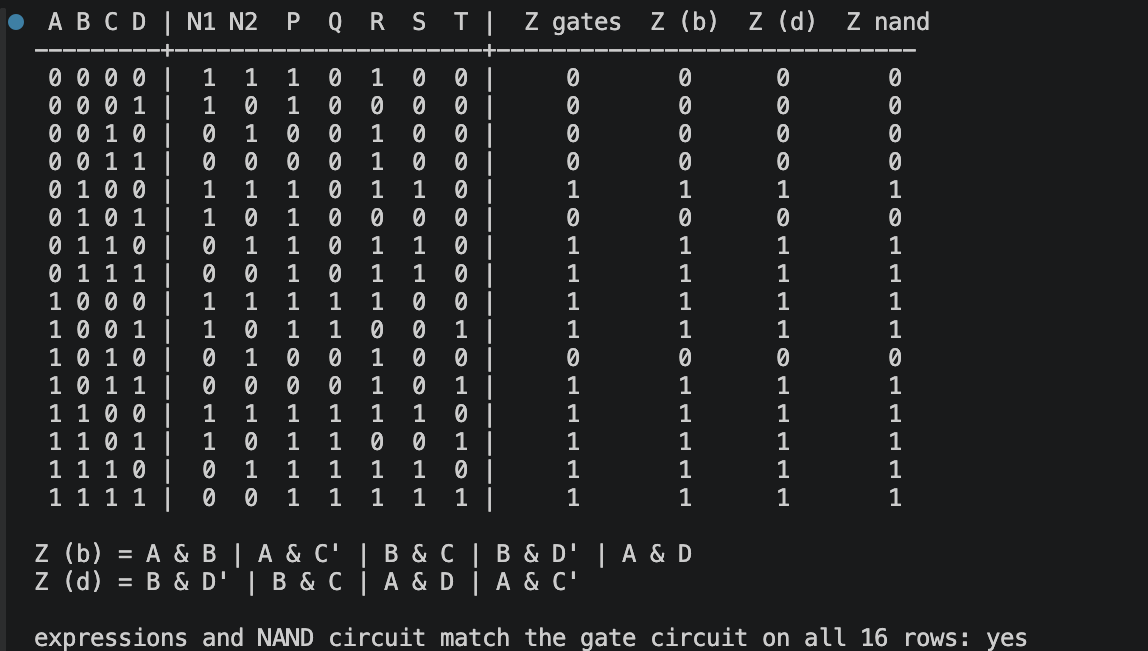
\includegraphics[width=0.78\linewidth]{q2_output.png}
\end{minipage}

\end{document}
